
\usetikzlibrary{shapes.geometric, arrows, decorations.markings}

\tikzstyle{vecArrow} = [thick, decoration={markings,mark=at position
   1 with {\arrow[semithick]{open triangle 60}}},
   double distance=1.4pt, shorten >= 5.5pt,
   preaction = {decorate},
   postaction = {draw,line width=1.4pt, white,shorten >= 4.5pt}]

\tikzstyle{entity} = [rectangle, minimum width=3cm, minimum height=1cm,
                      text width=3cm,
                      fill=white,
                      draw=black,
                      text centered,
                      top color=gray,
                      opacity=0.5,
                      bottom color=white]
                      
\tikzstyle{relationship} = [diamond, minimum width=3cm, minimum height=1cm,
                      text width=3cm,
                      fill=white,
                      draw=black]

\tikzstyle{attribute} = [rectangle, minimum width=3cm, minimum height=1cm,
                      text width=3cm,
                      fill=white,
                      draw=black]
                      

% \tikzstyle{attribute} = [top color=white, bottom color=yellow!20, 
%                                draw=yellow, node distance=1cm]
\tikzstyle{isa} = [top color=white, bottom color=green!20, 
                         draw=green!50!black!100]


\centering
\scalebox{.5}{
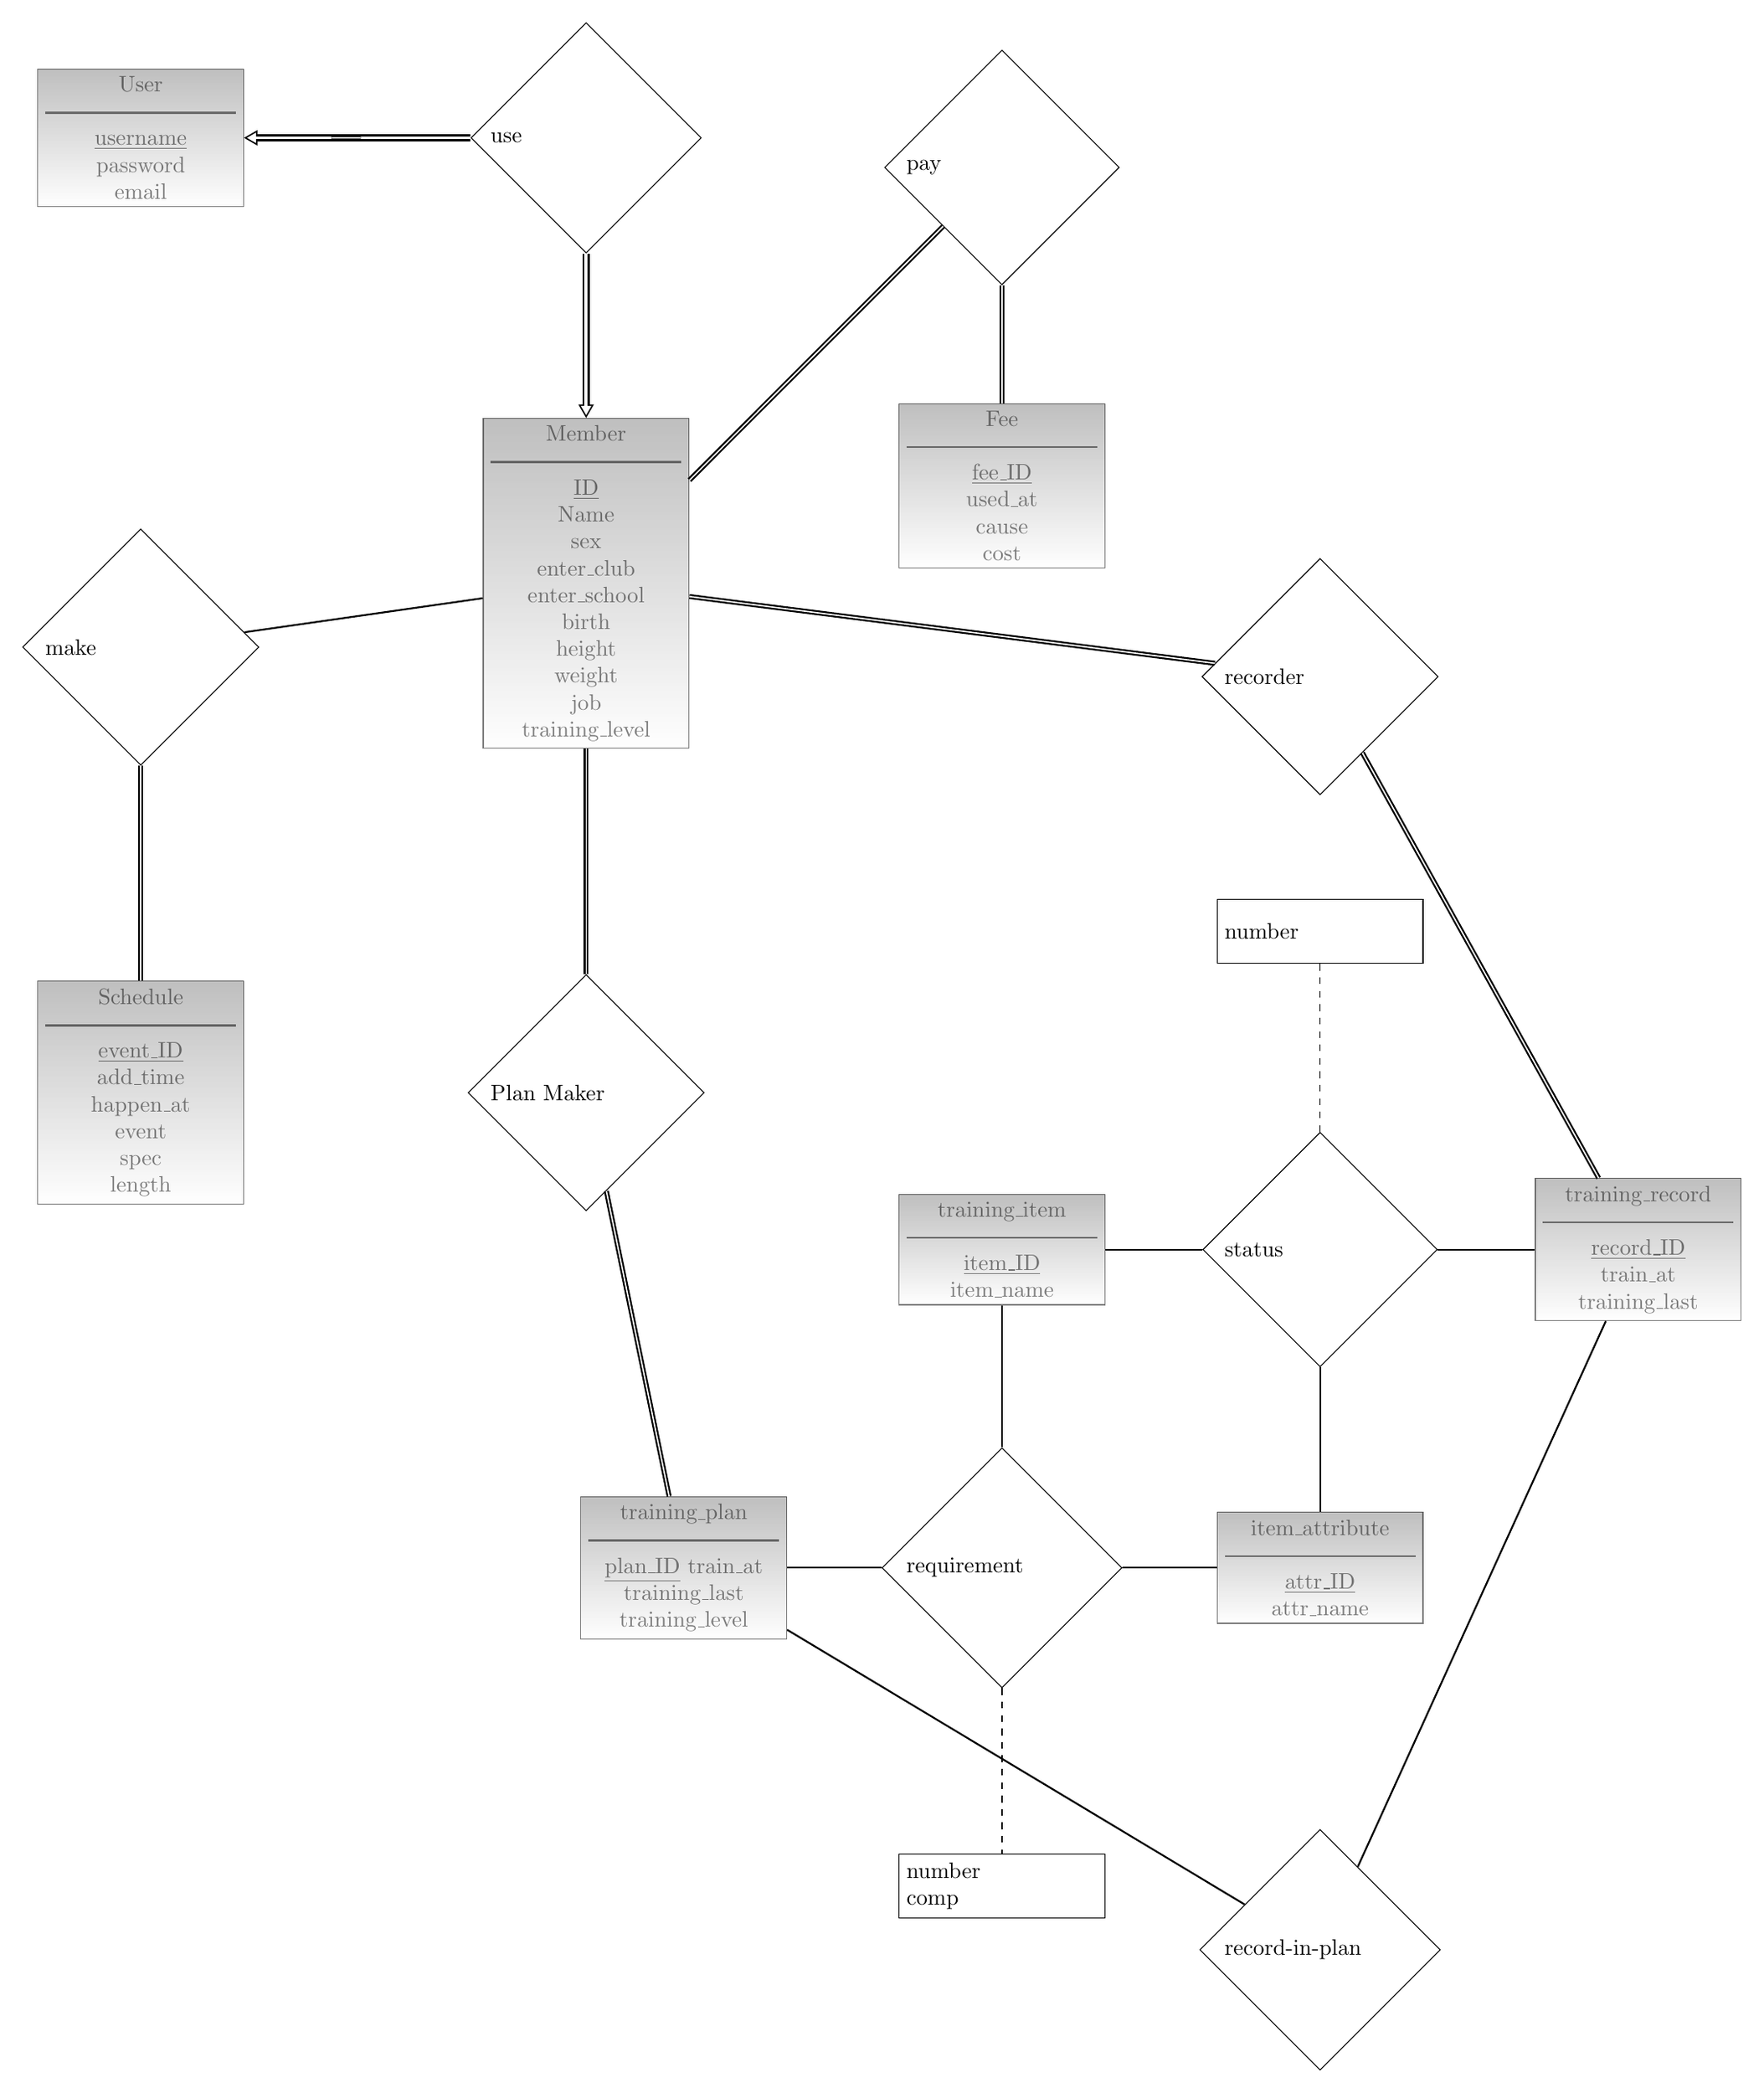
\begin{tikzpicture}[node distance=5cm]

  \node (user) [entity, xshift=-3cm] {
    User\\
    \noindent\rule[0.5ex]{3cm}{1pt}
    
    \underline{username}\\
    password\\
    email\\
  };

  \node (use) [relationship, right of=user, xshift=2cm] {
    use
  };

  \node (member) [entity, below of=use, yshift=-2cm] {
    Member \\
    \noindent\rule[0.5ex]{3cm}{1pt}

    \underline{ID}\\
    Name\\
    sex\\
    enter\_club\\
    enter\_school\\
    birth\\
    height\\
    weight\\
    job\\
    training\_level\\
  };

  \draw[vecArrow] (use) to (user);
  \draw[vecArrow] (use) to (member);

  %   \draw[thick, double](0,0)--(3ex,0) (use) to (user);
  % \draw[thick, double](0,0)--(3ex,0) (use) to (member);


  \node (schedule) [entity, below of=user, yshift=-10cm] {
    Schedule\\
    \noindent\rule[0.5ex]{3cm}{1pt}

    \underline{event\_ID}\\
    add\_time\\
    happen\_at\\
    event\\
    spec\\
    length\\
  };

  \node (make) [relationship, below of=user, yshift=-3cm] {
    make
  };

  \draw[thick, double](0,0)--(3ex,0) (make) to (schedule);
  \draw[thick] (make) to (member);

  \node(pay) [relationship, above right of=member, xshift=3cm, yshift=3cm] {
    pay
  };

  \node (fee) [entity, below of=pay] {
    Fee\\
    \noindent\rule[0.5ex]{3cm}{1pt}

    \underline{fee\_ID}\\
    used\_at\\
    cause\\
    cost\\
  };


  \draw[thick, double](0,0)--(3ex,0) (pay) to (fee);
  \draw[thick, double](0,0)--(3ex,0) (pay) to (member);

  \node (item) [entity, below of=fee, yshift=-7cm] {
    training\_item\\
    \noindent\rule[0.5ex]{3cm}{1pt}
    
    \underline{item\_ID}\\
    item\_name\\
  };

  \node(requirement) [relationship, below of=item] {
    requirement
  };

  \node(status) [relationship, right of=item] {
    status
  };

  \node(req-attr) [attribute, below of=requirement] {
    number\\
    comp
  };

  \node(sta-attr) [attribute, above of=status] {
    number\\
  };

  \node (record) [entity, right of=status] {
    training\_record\\
    \noindent\rule[0.5ex]{3cm}{1pt}

    \underline{record\_ID}\\
    train\_at\\
    training\_last\\
  };

  \node (plan) [entity, left of=requirement] {
    training\_plan\\
    \noindent\rule[0.5ex]{3cm}{1pt}
    
    \underline{plan\_ID}
    train\_at\\
    training\_last\\
    training\_level\\ % take note here, need changes
  };

  \node (attribute) [entity, right of=requirement] {
    item\_attribute\\
    \noindent\rule[0.5ex]{3cm}{1pt}

    \underline{attr\_ID}\\
    attr\_name\\
  };

  \draw[thick] (requirement) to (plan);
  \draw[thick] (requirement) to (item);
  \draw[thick] (requirement) to (attribute);

  \draw[thick] (status) to (item);
  \draw[thick] (status) to (attribute);
  \draw[thick] (status) to (record);
  
  \draw[dashed] (requirement) to (req-attr);
  \draw[dashed] (status) to (sta-attr);

  \node(plan-maker) [relationship, below of=member, yshift=-3cm] {
    Plan Maker
  };

  \node(recorder) [relationship, right of=fee, yshift=-3cm] {
    recorder
  };

  \draw[thick, double](0,0)--(3ex,0) (plan-maker) to (plan);
  \draw[thick, double](0,0)--(3ex,0) (plan-maker) to (member);

  \draw[thick, double](0,0)--(3ex,0) (recorder) to (record);
  \draw[thick, double](0,0)--(3ex,0) (recorder) to (member);
  
  \node(record-in-plan) [relationship, below of=attribute, yshift=-1cm] {
    record-in-plan
  };

  \draw[thick] (record-in-plan) to (record);
  \draw[thick] (record-in-plan) to (plan);

  % \node(ship) [entity] {
  %   ship\\
  %   \noindent\rule[0.5ex]{3cm}{1pt}
    
  %   \underline{name}\\
  %   condition\\
  % };

  % \node(ship type) [entity, right of=ship] {
  %   ship\_type\\
  %   \noindent\rule[0.5ex]{3cm}{1pt}

  %   type\_ID\\
  %   ship\_type\_name\\
  % };
      
\end{tikzpicture}
}